\ifdefined\beamerclass
\else
    \def\beamerclass{beamer}
\fi
\documentclass[\beamerclass]{beamer}

\usepackage{pgfpages}
\mode<handout>{
	% \setbeamercolor{background canvas}{bg=black!20}
	\pgfpagesuselayout{2 on 1}[a4paper,border shrink=5mm]
}

\usepackage{lmodern}
\usepackage{listings}
\usepackage{amsmath}
\usepackage{bm}
\usepackage{textpos} % package for the positioning

\usepackage{pgf, tikz}
\usetikzlibrary{arrows, automata}

\usetheme{Copenhagen}
\hypersetup{pdfstartview={Fit}}
\lstset{basicstyle=\small\ttfamily,breaklines=true}

\title[COMP6248 Deep Learning]{COMP6248 Differentiable Programming}
\subtitle{(and some Deep Learning)}
\author{Jonathon Hare}
\institute[]
{
  Vision, Learning and Control\\
  University of Southampton 
}
\date{}
\subject{Computer Science}
\useoutertheme{infolines}
\setbeamertemplate{headline}{} %remove headline
\setbeamertemplate{navigation symbols}{} %remove navigation symbols

\definecolor{darkblue}{RGB}{37,55,97}
\definecolor{mellowyellow}{RGB}{247,206,70}

\addtobeamertemplate{footnote}{\hskip -2em}{}
\newcommand\blfootnote[1]{%
  \begingroup
  \renewcommand\thefootnote{}\footnote{#1}%
  \addtocounter{footnote}{-1}%
  \endgroup
}

\begin{document}

\begin{frame}[plain]
        \begin{tikzpicture}[overlay, remember picture, shift={(current page.south west)},font={\fontfamily{Montserrat-TOsF}\selectfont}]
        \fill [mellowyellow,text=darkblue] (0,0) rectangle (\paperwidth, \paperheight);
        \draw (4,7) node [align=left,text=darkblue] {\Huge \begin{tabular}{l} \textbf{Differentiate} \\ \textbf{your} \\ \textbf{Objective} \end{tabular}};
        \draw (11,1) node [align=left,text=darkblue] {\includegraphics[scale=0.15]{../vlc.png}};
        \end{tikzpicture}
\end{frame}

\frame{
  \titlepage
}

\begin{frame}
\frametitle{Remaining lectures}

\begin{itemize}
	\item<+-> The following topics will be covered as full 45-minute video lectures:
	\begin{itemize}
		\item Embeddings
		\item Auto-encoders, unsupervised learning and self-supervision
		\item Differentiable relaxations and reparameterisations
		\item Generative Models
	\end{itemize}
	\item<+-> Some assorted topics will also be covered in shorter videos.
	\item<+-> You'll be able to ask questions via Teams and Slack. We'll also experiment with a live Q\&A session using Blackboard Collaborate.
	\item<+-> All the video content is on Blackboard (but perhaps more usefully linked directly from the module page).
\end{itemize}
\end{frame}

\begin{frame}[plain]
\begin{tikzpicture}[remember picture,overlay]
        \node[at=(current page.center)] {
            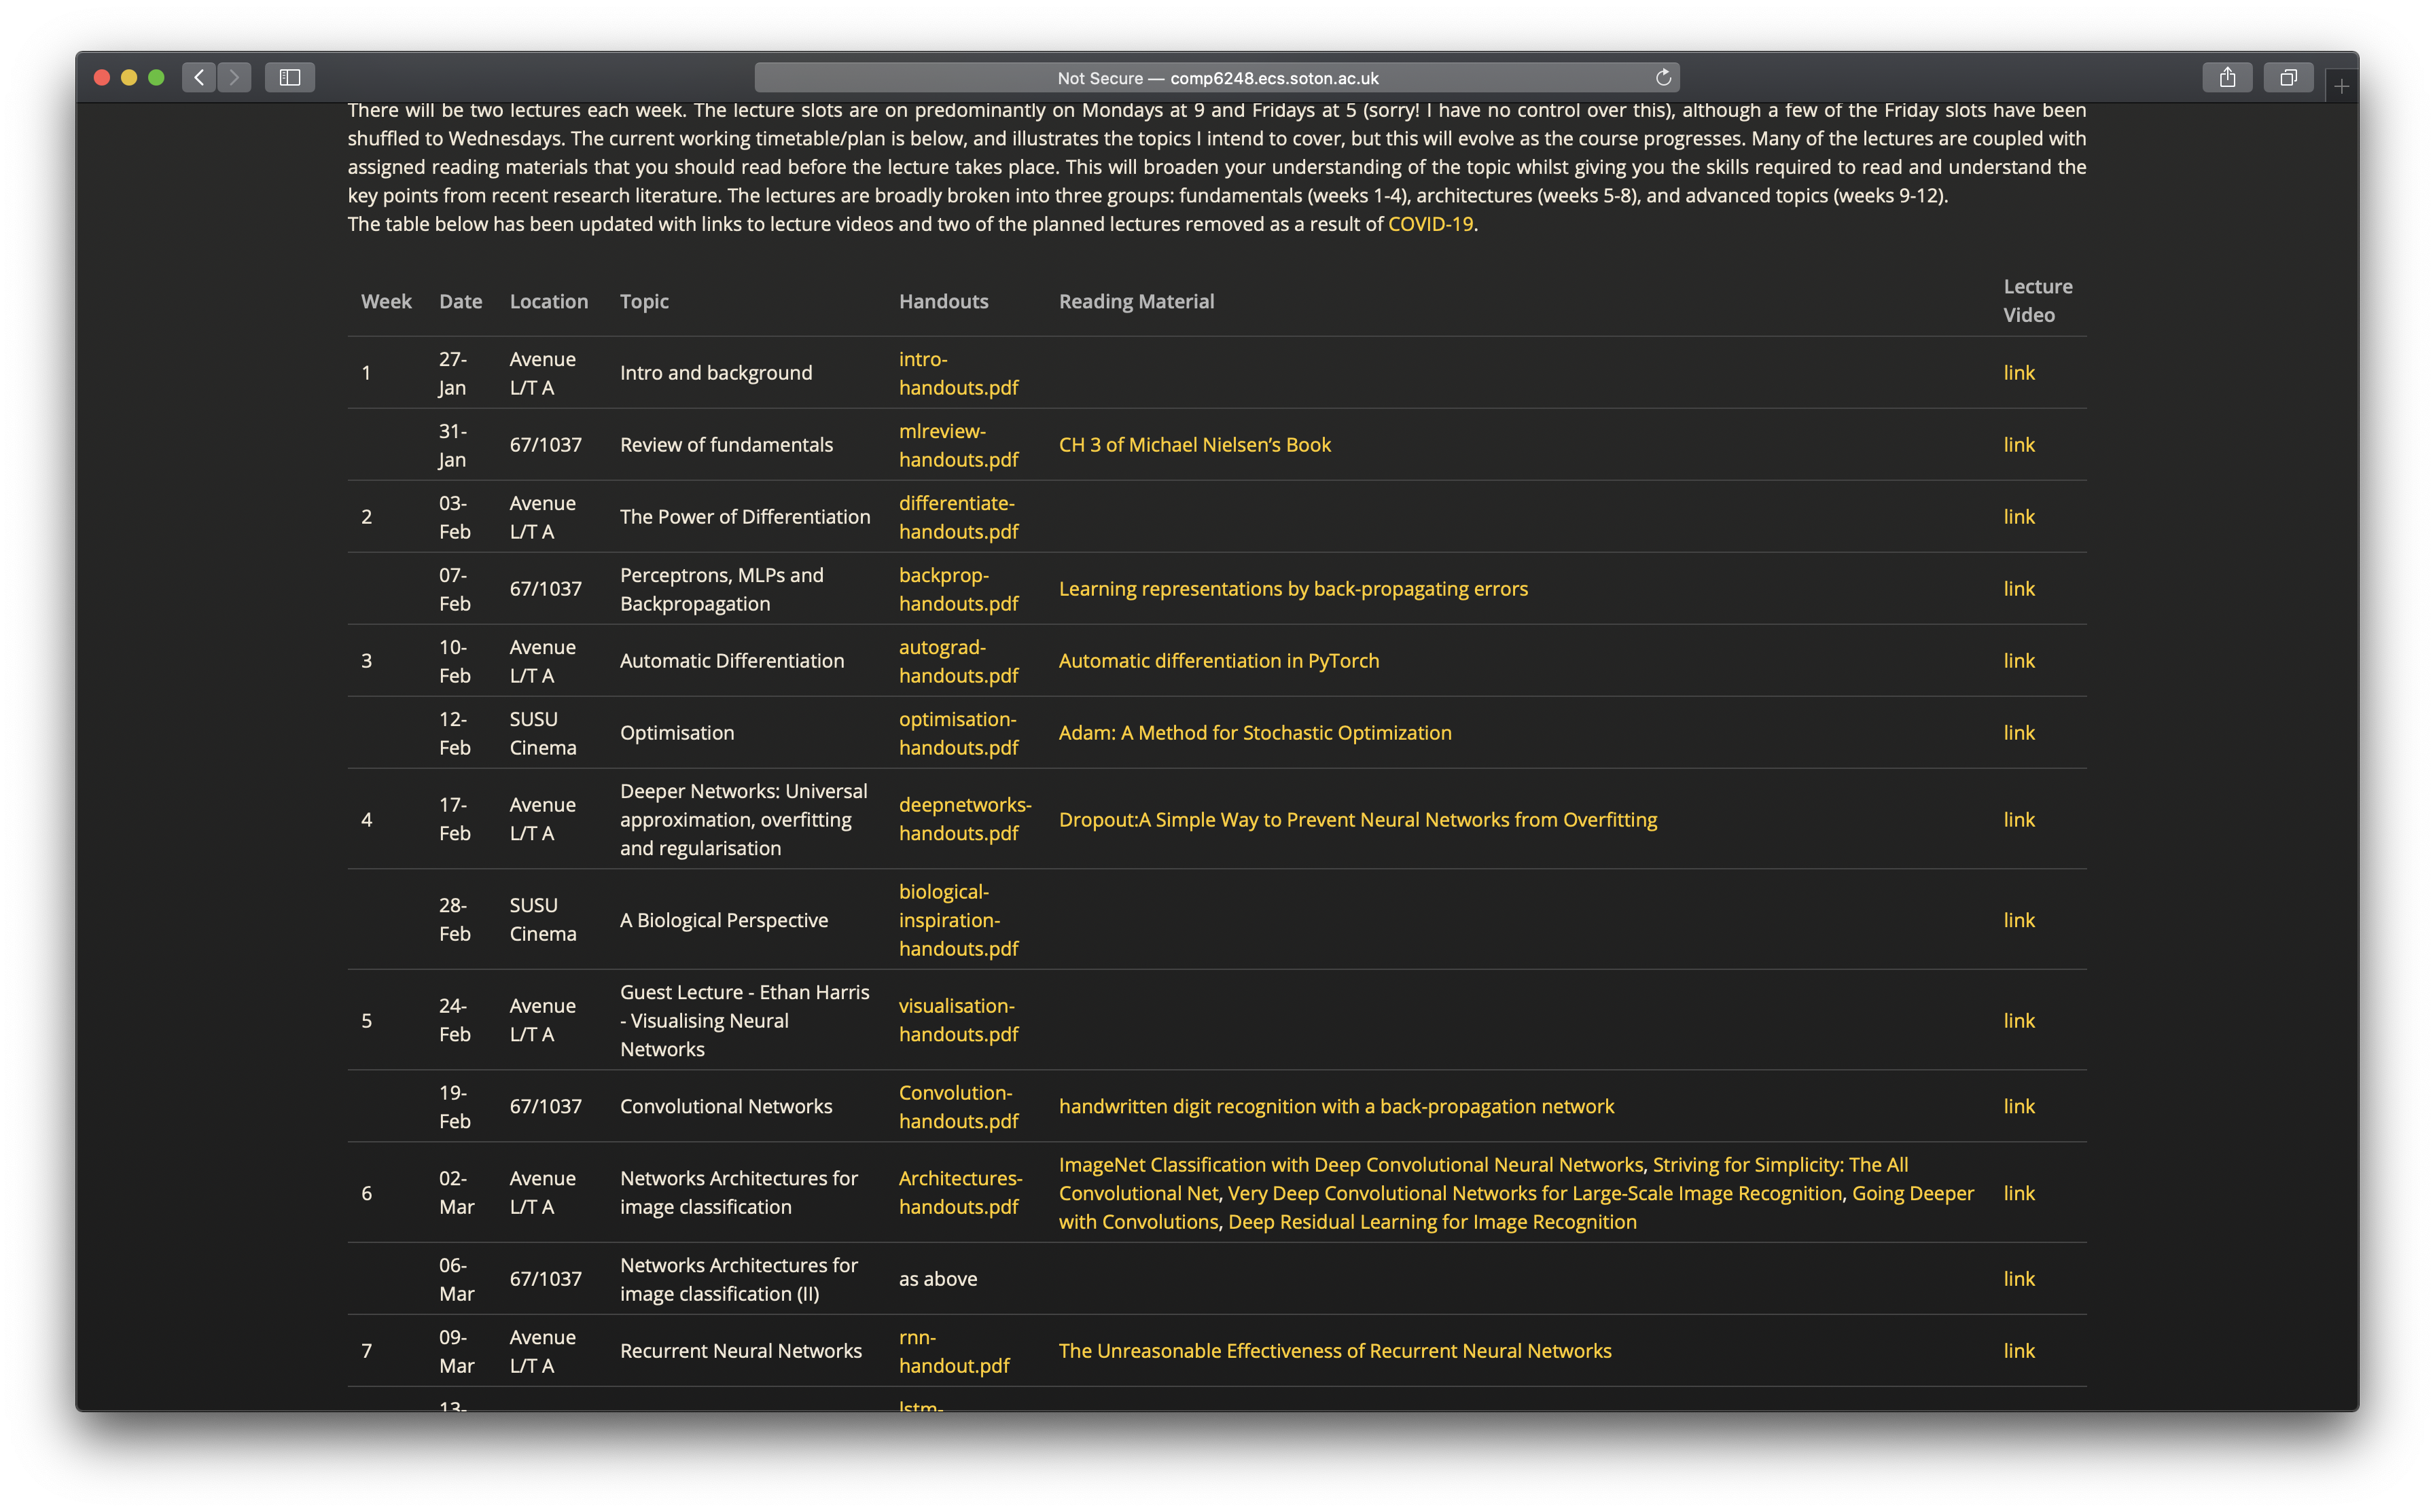
\includegraphics[scale=0.28]{webpage}
        };
    \end{tikzpicture}
\end{frame}


\begin{frame}
\frametitle{Remaining labs}
% There are still three lab sessions outstanding. These will run virtually (using either Google colab, ECS's remote GPU service or the student's own machine) at the normal scheduled time. The PhD demonstrator team will be asked to be live on the Slack and Teams channels to answer questions and talk to any students that need help. The lab timetable has been updated to restart from the 29th April for three weeks.

% The assessed lab exercises will be made available for the start of each lab as is currently being done. The deadline for handin has been moved to the 20th May. 
\begin{itemize}
	\item<+-> Labs will run as before starting on the Wednesday 29th April for three weeks.
	\item<+-> Demonstrators will be available in Teams and Slack during the normal lab hours (9-11 AM BST).
	\item<+-> You can use colab or log onto lab machines remotely if you want to.
	\item<+-> New handin date for lab exercises: 20th May.
\end{itemize}
\end{frame}

\begin{frame}
\frametitle{Online quiz 2}
% This should run in pretty much the same way the first one did (using blackboard) - rescheduled to the 14th May.
\begin{itemize}
	\item New (proposed) date: Thursday 14th May.
	\item As before you'll have 1 hour to complete it.
	\item I'll keep it open to start for 24 hours this time.
\end{itemize}
\end{frame}

\begin{frame}
\frametitle{Group Coursework}

\begin{itemize}
	\item<+-> Continue as before...
	\item<+-> Ask the demonstrators or me questions during the online lab sessions.
	\item<+-> The deadline will be extended to the 16:00 on the 29th May. 
\end{itemize}

\end{frame}
\end{document}